\section{CVariable\-Binding$<$ T $>$  Class Template Reference}
\label{classCVariableBinding}\index{CVariableBinding@{CVariable\-Binding}}
{\tt \#include $<$CVariable\-Binding.h$>$}

Inheritance diagram for CVariable\-Binding$<$ T $>$::\begin{figure}[H]
\begin{center}
\leavevmode
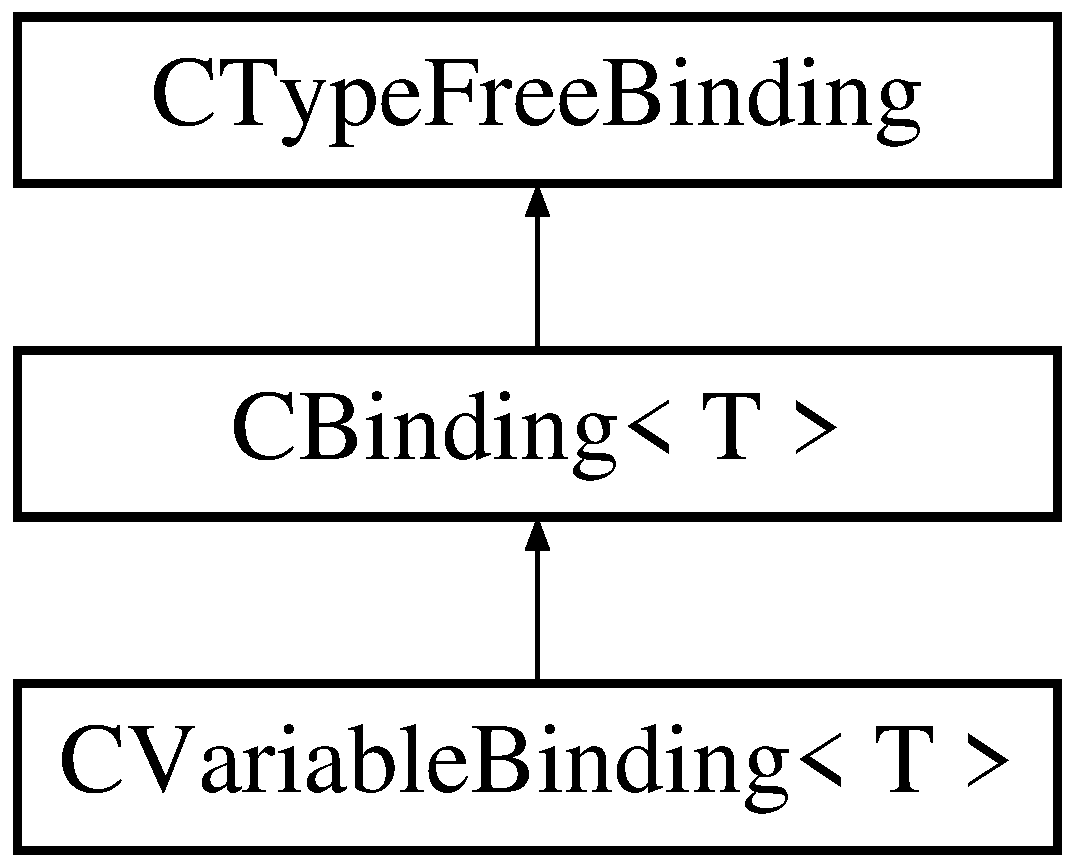
\includegraphics[height=3cm]{classCVariableBinding}
\end{center}
\end{figure}
\subsection*{Public Methods}
\begin{CompactItemize}
\item 
{\bf CVariable\-Binding} (T \&variable, const string \&r\-Name, T t\-Initial\-Value)
\item 
{\bf CVariable\-Binding} (T \&variable, const char $\ast$p\-Name, T t\-Initial\-Value)
\item 
{\bf $\sim$CVariable\-Binding} ()
\item 
T {\bf get\-Variable} () const
\item 
string {\bf get\-Name} () const
\item 
T {\bf get\-Init\-Value} () const
\item 
int {\bf get\-Var\-Type} () const
\item 
void {\bf set\-Variable} (T value)
\item 
void {\bf set\-Pointer} (T $\ast$ptr)
\item 
void {\bf set\-Name} (const string \&r\-Name)
\item 
void {\bf set\-Name} (const char $\ast$p\-Name)
\item 
void {\bf set\-Initial\-Value} (T value)
\item 
void {\bf set\-Variable\-Type} (int type)
\item 
virtual void {\bf Init\-Bindings} ({\bf CTCLInterpreter} \&r\-Interp)
\item 
virtual void {\bf Commit} ({\bf CTCLInterpreter} \&r\-Interp)
\item 
virtual void {\bf Shutdown\-Bindings} ({\bf CTCLInterpreter} \&r\-Interp)
\item 
virtual void {\bf Dump} (int fd)
\end{CompactItemize}
\subsection*{Private Methods}
\begin{CompactItemize}
\item 
{\bf CVariable\-Binding} (const CVariable\-Binding \&r\-Binding)
\item 
CVariable\-Binding \& {\bf operator=} (const CVariable\-Binding \&r\-Binding)
\item 
int {\bf operator==} (const CVariable\-Binding \&r\-Binding)
\end{CompactItemize}
\subsection*{Private Attributes}
\begin{CompactItemize}
\item 
T $\ast$ {\bf m\_\-p\-Variable}
\begin{CompactList}\small\item\em Pointer to the config variable.\item\end{CompactList}\item 
string {\bf m\_\-s\-Name}
\begin{CompactList}\small\item\em Name of the variable (for Tcl binding).\item\end{CompactList}\item 
T {\bf m\_\-t\-Initial\-Value}
\begin{CompactList}\small\item\em Initial value of the variable.\item\end{CompactList}\item 
int {\bf m\_\-TCLVariable\-Type}
\begin{CompactList}\small\item\em Type of binding (for TCL).\item\end{CompactList}\end{CompactItemize}


\subsection{Detailed Description}
\subsubsection*{template$<$class T$>$ class CVariable\-Binding$<$ T $>$}

CVariable\-Binding is a class which encapsulates a configuration scalar variable. The Variable is maintained by the user of this class. The Init\-Bindings makes a link to the variable. The Commit does nothing The Shutdown\-Bindings member removes the link. 



Definition at line 316 of file CVariable\-Binding.h.

\subsection{Constructor \& Destructor Documentation}
\index{CVariableBinding@{CVariable\-Binding}!CVariableBinding@{CVariableBinding}}
\index{CVariableBinding@{CVariableBinding}!CVariableBinding@{CVariable\-Binding}}
\subsubsection{\setlength{\rightskip}{0pt plus 5cm}template$<$class T$>$ CVariable\-Binding$<$ T $>$::CVariable\-Binding (T \& {\em variable}, const string \& {\em rname}, T {\em t\-Initial\-Value})}\label{classCVariableBinding_a0}


Construct a variable binding from the variable, a name, and initial value. The name is expressed as a string:\begin{Desc}
\item[Parameters: ]\par
\begin{description}
\item[{\em 
variable}]- reference to the variable to bind. \item[{\em 
rname}]- Reference to the string containing the name of the TCL variable which will be bound. \item[{\em 
t\-Initial\-Value}]- Initial value to give the variable prior to  reading the config file.. a default. \end{description}
\end{Desc}


Definition at line 308 of file CVariable\-Binding.cpp.\index{CVariableBinding@{CVariable\-Binding}!CVariableBinding@{CVariableBinding}}
\index{CVariableBinding@{CVariableBinding}!CVariableBinding@{CVariable\-Binding}}
\subsubsection{\setlength{\rightskip}{0pt plus 5cm}template$<$class T$>$ CVariable\-Binding$<$ T $>$::CVariable\-Binding (T \& {\em variable}, const char $\ast$ {\em p\-Name}, T {\em t\-Initial\-Value})}\label{classCVariableBinding_a1}


Construct a variable binding from the variable reference asciz string pointer and initial value:\begin{Desc}
\item[Parameters: ]\par
\begin{description}
\item[{\em 
variable}]- Reference to the variable to configure. \item[{\em 
p\-Name}]- Reference to char$\ast$ string to give name. \item[{\em 
t\-Initial\-Value}]- Initial value to give to the variable. \end{description}
\end{Desc}


Definition at line 325 of file CVariable\-Binding.cpp.\index{CVariableBinding@{CVariable\-Binding}!~CVariableBinding@{$\sim$CVariableBinding}}
\index{~CVariableBinding@{$\sim$CVariableBinding}!CVariableBinding@{CVariable\-Binding}}
\subsubsection{\setlength{\rightskip}{0pt plus 5cm}template$<$class T$>$ CVariable\-Binding$<$ T $>$::$\sim$CVariable\-Binding ()\hspace{0.3cm}{\tt  [inline]}}\label{classCVariableBinding_a2}




Definition at line 326 of file CVariable\-Binding.h.\index{CVariableBinding@{CVariable\-Binding}!CVariableBinding@{CVariableBinding}}
\index{CVariableBinding@{CVariableBinding}!CVariableBinding@{CVariable\-Binding}}
\subsubsection{\setlength{\rightskip}{0pt plus 5cm}template$<$class T$>$ CVariable\-Binding$<$ T $>$::CVariable\-Binding (const CVariable\-Binding$<$ T $>$ \& {\em r\-Binding})\hspace{0.3cm}{\tt  [private]}}\label{classCVariableBinding_c0}




\subsection{Member Function Documentation}
\index{CVariableBinding@{CVariable\-Binding}!Commit@{Commit}}
\index{Commit@{Commit}!CVariableBinding@{CVariable\-Binding}}
\subsubsection{\setlength{\rightskip}{0pt plus 5cm}template$<$class T$>$ void CVariable\-Binding$<$ T $>$::Commit ({\bf CTCLInterpreter} \& {\em r\-Interp})\hspace{0.3cm}{\tt  [virtual]}}\label{classCVariableBinding_a14}


Commit - no commit operation is required. Since the variable was linked, it already has any changed value.\begin{Desc}
\item[Parameters: ]\par
\begin{description}
\item[{\em 
r\-Interp}]- The interpreter which read in the config file. \end{description}
\end{Desc}


Implements {\bf CBinding$<$ T $>$} {\rm (p.\,\pageref{classCBinding_a1})}.

Definition at line 357 of file CVariable\-Binding.cpp.\index{CVariableBinding@{CVariable\-Binding}!Dump@{Dump}}
\index{Dump@{Dump}!CVariableBinding@{CVariable\-Binding}}
\subsubsection{\setlength{\rightskip}{0pt plus 5cm}template$<$class T$>$ void CVariable\-Binding$<$ T $>$::Dump (int {\em fd})\hspace{0.3cm}{\tt  [virtual]}}\label{classCVariableBinding_a16}


This function is called just prior to deleting the interpreter. Any cleanup actions required by the binding should be done at this point. For example, if Init mapped a C variable to a TCL variable, that mapping should be broken. \begin{Desc}
\item[Parameters: ]\par
\begin{description}
\item[{\em 
r\-Interp}]- The interpreter about to be deleted. virtual void {\bf Shutdown\-Bindings}(CTCLInterpreter\& r\-Interp) {\rm (p.\,\pageref{classCVariableBinding_a15})}= 0; /$\ast$! This function is called to write the set of Tcl commands required to duplicate the current state. Note that this may not be identical to the set of commands which produced the configuration. \end{description}
\end{Desc}


Implements {\bf CBinding$<$ T $>$} {\rm (p.\,\pageref{classCBinding_a2})}.

Definition at line 386 of file CVariable\-Binding.cpp.

References CTCLString::Append\-Element(), CBinding$<$ T $>$::Item\-To\-String(), CVariable\-Binding$<$ T $>$::m\_\-p\-Variable, and CVariable\-Binding$<$ T $>$::m\_\-s\-Name.\index{CVariableBinding@{CVariable\-Binding}!getInitValue@{getInitValue}}
\index{getInitValue@{getInitValue}!CVariableBinding@{CVariable\-Binding}}
\subsubsection{\setlength{\rightskip}{0pt plus 5cm}template$<$class T$>$ T CVariable\-Binding$<$ T $>$::get\-Init\-Value () const\hspace{0.3cm}{\tt  [inline]}}\label{classCVariableBinding_a5}




Definition at line 342 of file CVariable\-Binding.h.

References CVariable\-Binding$<$ T $>$::m\_\-t\-Initial\-Value.\index{CVariableBinding@{CVariable\-Binding}!getName@{getName}}
\index{getName@{getName}!CVariableBinding@{CVariable\-Binding}}
\subsubsection{\setlength{\rightskip}{0pt plus 5cm}template$<$class T$>$ string CVariable\-Binding$<$ T $>$::get\-Name () const\hspace{0.3cm}{\tt  [inline]}}\label{classCVariableBinding_a4}




Definition at line 339 of file CVariable\-Binding.h.

References CVariable\-Binding$<$ T $>$::m\_\-s\-Name.\index{CVariableBinding@{CVariable\-Binding}!getVariable@{getVariable}}
\index{getVariable@{getVariable}!CVariableBinding@{CVariable\-Binding}}
\subsubsection{\setlength{\rightskip}{0pt plus 5cm}template$<$class T$>$ T CVariable\-Binding$<$ T $>$::get\-Variable () const\hspace{0.3cm}{\tt  [inline]}}\label{classCVariableBinding_a3}




Definition at line 336 of file CVariable\-Binding.h.

References CVariable\-Binding$<$ T $>$::m\_\-p\-Variable.\index{CVariableBinding@{CVariable\-Binding}!getVarType@{getVarType}}
\index{getVarType@{getVarType}!CVariableBinding@{CVariable\-Binding}}
\subsubsection{\setlength{\rightskip}{0pt plus 5cm}template$<$class T$>$ int CVariable\-Binding$<$ T $>$::get\-Var\-Type () const\hspace{0.3cm}{\tt  [inline]}}\label{classCVariableBinding_a6}




Definition at line 345 of file CVariable\-Binding.h.

References CVariable\-Binding$<$ T $>$::m\_\-TCLVariable\-Type.\index{CVariableBinding@{CVariable\-Binding}!InitBindings@{InitBindings}}
\index{InitBindings@{InitBindings}!CVariableBinding@{CVariable\-Binding}}
\subsubsection{\setlength{\rightskip}{0pt plus 5cm}template$<$class T$>$ void CVariable\-Binding$<$ T $>$::Init\-Bindings ({\bf CTCLInterpreter} \& {\em r\-Interp})\hspace{0.3cm}{\tt  [virtual]}}\label{classCVariableBinding_a13}


Initialize bindings prior to reading the configuration file. In this case, the TCL variable is bound to the thing referenced by the m\_\-p\-Variable pointer. \begin{Desc}
\item[Parameters: ]\par
\begin{description}
\item[{\em 
r\-Interp}]- The interpreter which will be used to read the config file. \end{description}
\end{Desc}


Implements {\bf CBinding$<$ T $>$} {\rm (p.\,\pageref{classCBinding_a0})}.

Definition at line 341 of file CVariable\-Binding.cpp.

References CTCLInterpreter::get\-Interpreter(), CVariable\-Binding$<$ T $>$::m\_\-p\-Variable, CVariable\-Binding$<$ T $>$::m\_\-s\-Name, CVariable\-Binding$<$ T $>$::m\_\-TCLVariable\-Type, and CVariable\-Binding$<$ T $>$::m\_\-t\-Initial\-Value.\index{CVariableBinding@{CVariable\-Binding}!operator=@{operator=}}
\index{operator=@{operator=}!CVariableBinding@{CVariable\-Binding}}
\subsubsection{\setlength{\rightskip}{0pt plus 5cm}template$<$class T$>$ CVariable\-Binding\& CVariable\-Binding$<$ T $>$::operator= (const CVariable\-Binding$<$ T $>$ \& {\em r\-Binding})\hspace{0.3cm}{\tt  [private]}}\label{classCVariableBinding_c1}


\index{CVariableBinding@{CVariable\-Binding}!operator==@{operator==}}
\index{operator==@{operator==}!CVariableBinding@{CVariable\-Binding}}
\subsubsection{\setlength{\rightskip}{0pt plus 5cm}template$<$class T$>$ int CVariable\-Binding$<$ T $>$::operator== (const CVariable\-Binding$<$ T $>$ \& {\em r\-Binding})\hspace{0.3cm}{\tt  [private]}}\label{classCVariableBinding_c2}


\index{CVariableBinding@{CVariable\-Binding}!setInitialValue@{setInitialValue}}
\index{setInitialValue@{setInitialValue}!CVariableBinding@{CVariable\-Binding}}
\subsubsection{\setlength{\rightskip}{0pt plus 5cm}template$<$class T$>$ void CVariable\-Binding$<$ T $>$::set\-Initial\-Value (T {\em value})\hspace{0.3cm}{\tt  [inline]}}\label{classCVariableBinding_a11}




Definition at line 362 of file CVariable\-Binding.h.

References CVariable\-Binding$<$ T $>$::m\_\-t\-Initial\-Value.\index{CVariableBinding@{CVariable\-Binding}!setName@{setName}}
\index{setName@{setName}!CVariableBinding@{CVariable\-Binding}}
\subsubsection{\setlength{\rightskip}{0pt plus 5cm}template$<$class T$>$ void CVariable\-Binding$<$ T $>$::set\-Name (const char $\ast$ {\em p\-Name})\hspace{0.3cm}{\tt  [inline]}}\label{classCVariableBinding_a10}




Definition at line 359 of file CVariable\-Binding.h.

References CVariable\-Binding$<$ T $>$::m\_\-s\-Name.\index{CVariableBinding@{CVariable\-Binding}!setName@{setName}}
\index{setName@{setName}!CVariableBinding@{CVariable\-Binding}}
\subsubsection{\setlength{\rightskip}{0pt plus 5cm}template$<$class T$>$ void CVariable\-Binding$<$ T $>$::set\-Name (const string \& {\em r\-Name})\hspace{0.3cm}{\tt  [inline]}}\label{classCVariableBinding_a9}




Definition at line 356 of file CVariable\-Binding.h.

References CVariable\-Binding$<$ T $>$::m\_\-s\-Name.\index{CVariableBinding@{CVariable\-Binding}!setPointer@{setPointer}}
\index{setPointer@{setPointer}!CVariableBinding@{CVariable\-Binding}}
\subsubsection{\setlength{\rightskip}{0pt plus 5cm}template$<$class T$>$ void CVariable\-Binding$<$ T $>$::set\-Pointer (T $\ast$ {\em ptr})\hspace{0.3cm}{\tt  [inline]}}\label{classCVariableBinding_a8}




Definition at line 353 of file CVariable\-Binding.h.

References CVariable\-Binding$<$ T $>$::m\_\-p\-Variable.\index{CVariableBinding@{CVariable\-Binding}!setVariable@{setVariable}}
\index{setVariable@{setVariable}!CVariableBinding@{CVariable\-Binding}}
\subsubsection{\setlength{\rightskip}{0pt plus 5cm}template$<$class T$>$ void CVariable\-Binding$<$ T $>$::set\-Variable (T {\em value})\hspace{0.3cm}{\tt  [inline]}}\label{classCVariableBinding_a7}




Definition at line 350 of file CVariable\-Binding.h.

References CVariable\-Binding$<$ T $>$::m\_\-p\-Variable.\index{CVariableBinding@{CVariable\-Binding}!setVariableType@{setVariableType}}
\index{setVariableType@{setVariableType}!CVariableBinding@{CVariable\-Binding}}
\subsubsection{\setlength{\rightskip}{0pt plus 5cm}template$<$class T$>$ void CVariable\-Binding$<$ T $>$::set\-Variable\-Type (int {\em type})\hspace{0.3cm}{\tt  [inline]}}\label{classCVariableBinding_a12}




Definition at line 365 of file CVariable\-Binding.h.

References CVariable\-Binding$<$ T $>$::m\_\-TCLVariable\-Type.\index{CVariableBinding@{CVariable\-Binding}!ShutdownBindings@{ShutdownBindings}}
\index{ShutdownBindings@{ShutdownBindings}!CVariableBinding@{CVariable\-Binding}}
\subsubsection{\setlength{\rightskip}{0pt plus 5cm}template$<$class T$>$ void CVariable\-Binding$<$ T $>$::Shutdown\-Bindings ({\bf CTCLInterpreter} \& {\em r\-Interp})\hspace{0.3cm}{\tt  [virtual]}}\label{classCVariableBinding_a15}




Implements {\bf CType\-Free\-Binding} {\rm (p.\,\pageref{classCTypeFreeBinding_a2})}.

Definition at line 366 of file CVariable\-Binding.cpp.

References CTCLInterpreter::get\-Interpreter(), and CVariable\-Binding$<$ T $>$::m\_\-s\-Name.

\subsection{Member Data Documentation}
\index{CVariableBinding@{CVariable\-Binding}!m_pVariable@{m\_\-pVariable}}
\index{m_pVariable@{m\_\-pVariable}!CVariableBinding@{CVariable\-Binding}}
\subsubsection{\setlength{\rightskip}{0pt plus 5cm}template$<$class T$>$ T$\ast$ CVariable\-Binding$<$ T $>$::m\_\-p\-Variable\hspace{0.3cm}{\tt  [private]}}\label{classCVariableBinding_o0}


Pointer to the config variable.



Definition at line 318 of file CVariable\-Binding.h.

Referenced by CVariable\-Binding$<$ T $>$::Dump(), CVariable\-Binding$<$ T $>$::get\-Variable(), CVariable\-Binding$<$ T $>$::Init\-Bindings(), CVariable\-Binding$<$ T $>$::set\-Pointer(), and CVariable\-Binding$<$ T $>$::set\-Variable().\index{CVariableBinding@{CVariable\-Binding}!m_sName@{m\_\-sName}}
\index{m_sName@{m\_\-sName}!CVariableBinding@{CVariable\-Binding}}
\subsubsection{\setlength{\rightskip}{0pt plus 5cm}template$<$class T$>$ string CVariable\-Binding$<$ T $>$::m\_\-s\-Name\hspace{0.3cm}{\tt  [private]}}\label{classCVariableBinding_o1}


Name of the variable (for Tcl binding).



Definition at line 319 of file CVariable\-Binding.h.

Referenced by CVariable\-Binding$<$ T $>$::Dump(), CVariable\-Binding$<$ T $>$::get\-Name(), CVariable\-Binding$<$ T $>$::Init\-Bindings(), CVariable\-Binding$<$ T $>$::set\-Name(), and CVariable\-Binding$<$ T $>$::Shutdown\-Bindings().\index{CVariableBinding@{CVariable\-Binding}!m_TCLVariableType@{m\_\-TCLVariableType}}
\index{m_TCLVariableType@{m\_\-TCLVariableType}!CVariableBinding@{CVariable\-Binding}}
\subsubsection{\setlength{\rightskip}{0pt plus 5cm}template$<$class T$>$ int CVariable\-Binding$<$ T $>$::m\_\-TCLVariable\-Type\hspace{0.3cm}{\tt  [private]}}\label{classCVariableBinding_o3}


Type of binding (for TCL).



Definition at line 321 of file CVariable\-Binding.h.

Referenced by CVariable\-Binding$<$ T $>$::get\-Var\-Type(), CVariable\-Binding$<$ T $>$::Init\-Bindings(), and CVariable\-Binding$<$ T $>$::set\-Variable\-Type().\index{CVariableBinding@{CVariable\-Binding}!m_tInitialValue@{m\_\-tInitialValue}}
\index{m_tInitialValue@{m\_\-tInitialValue}!CVariableBinding@{CVariable\-Binding}}
\subsubsection{\setlength{\rightskip}{0pt plus 5cm}template$<$class T$>$ T CVariable\-Binding$<$ T $>$::m\_\-t\-Initial\-Value\hspace{0.3cm}{\tt  [private]}}\label{classCVariableBinding_o2}


Initial value of the variable.



Definition at line 320 of file CVariable\-Binding.h.

Referenced by CVariable\-Binding$<$ T $>$::get\-Init\-Value(), CVariable\-Binding$<$ T $>$::Init\-Bindings(), and CVariable\-Binding$<$ T $>$::set\-Initial\-Value().

The documentation for this class was generated from the following files:\begin{CompactItemize}
\item 
{\bf CVariable\-Binding.h}\item 
{\bf CVariable\-Binding.cpp}\end{CompactItemize}
